\documentclass{beamer}
\usetheme{metropolis}

% specifications for presenter mode
%\beamerdefaultoverlayspecification{<+->}
%\setbeamercovered{transparent}

\usepackage[english]{babel}
\usepackage[utf8x]{inputenc}

%\usepackage{coloremoji}
\usepackage{layout}
\usepackage{multirow}
\usepackage{array}
\usepackage{graphicx}
\graphicspath{ {Figs/} }
\usepackage{animate}

\setbeameroption{hide notes}
\setbeamertemplate{note page}[plain]
\usepackage{listings}
\usepackage{datetime}
\usepackage{url}
\usepackage{tcolorbox}
\usepackage{appendixnumberbeamer}

\usepackage{tikz}
\def\checkmark{\tikz\fill[scale=0.4](0,.35) -- (.25,0) -- (1,.7) -- (.25,.15) -- cycle;}

% math shorthand
\usepackage{bm}
\usepackage{amstext}
\usepackage{amsthm}
\usepackage{amsmath}
\usepackage{mathtools}
\newcommand{\R}{\mathbb{R}}
\newcommand{\D}{\mathcal{D}}
\newcommand{\E}{\mathbb{E}}
\newcommand{\I}{\mathbb{I}}
\newcommand{\pr}{\mathbb{P}}
\newcommand{\F}{\mathcal{F}}
\newcommand{\X}{\mathcal{X}}
\newcommand{\M}{\mathcal{M}}
\newcommand{\lik}{\mathcal{L}}

\newtheorem*{assumption*}{\assumptionnumber}
\providecommand{\assumptionnumber}{}
\makeatletter
\newenvironment{assumption}[2]
 {%
  \renewcommand{\assumptionnumber}{Assumption #1: $\mathcal{#2}$}%
  \begin{assumption*}%
  \protected@edef\@currentlabel{#1: $\mathcal{#2}$}%
 }
 {%
  \end{assumption*}
 }
\makeatother

\DeclarePairedDelimiterX{\infdivx}[2]{(}{)}{%
  #1\;\delimsize\|\;#2%
}
\newcommand{\infdiv}{D\infdivx}
\DeclarePairedDelimiter{\norm}{\lVert}{\rVert}
\DeclareMathOperator*{\argmin}{arg\,min}
\DeclareMathOperator*{\argmax}{arg\,max}

% indepndence notation macro
\newcommand\indep{\protect\mathpalette{\protect\independenT}{\perp}}
\def\independenT#1#2{\mathrel{\rlap{$#1#2$}\mkern2mu{#1#2}}}

% Bibliography
\usepackage{natbib}
\bibpunct{(}{)}{,}{a}{}{;}
\usepackage{bibentry}

\title{\normalsize Vaccine efficacy assessment under two-phase sampling based on
  the causal effects of stochastic interventions}

\author{\href{https://nimahejazi.org}{Nima Hejazi}\\[-10pt]}

\institute{
  \begin{figure}[!htb]
    \centering
    \begin{minipage}{.65\textwidth}
        Graduate Group in Biostatistics, and \\
        Center for Computational Biology, \\
        University of California, Berkeley \\[6pt]
        
\includegraphics[scale=0.12]{twitter-icon.png}
          \href{https://twitter.com/nshejazi}{nshejazi} \\
        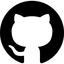
\includegraphics[scale=0.09]{github-icon.png}
          \href{https://github.com/nhejazi}{nhejazi} \\
        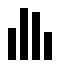
\includegraphics[scale=0.12]{homepage.png}
          \href{https://nimahejazi.org}{nimahejazi.org} \\
        
\includegraphics[scale=0.12]{pdf-icon.png}
        \href{https://bit.ly/2019\_sfasa\_jsm}{bit.ly/2019\_sfasa\_jsm} \\
        {\scriptsize joint work with David Benkeser and Mark van der Laan}
    \end{minipage}%
    \begin{minipage}{0.35\textwidth}
      \centering
      
\includegraphics[height=0.80in,width=0.80in]{ucberkeleyseal_874_540.eps}
    \end{minipage}
  \end{figure}
}

\date{Wednesday, 05 June 2019}

%%%%%%%%%%%%%%%%%%%%%%%%%%%%%%%%%%%%%%%%%%%%%%%%%%%%%%%%%%%%%%%%%%%%%%%%%%%%%%%%

\begin{document}

\begin{frame}[noframenumbering]
  \thispagestyle{empty}
  \titlepage
\end{frame}

%%%%%%%%%%%%%%%%%%%%%%%%%%%%%%%%%%%%%%%%%%%%%%%%%%%%%%%%%%%%%%%%%%%%%%%%%%%%%%%%

\begin{frame}[c]{The burden of HIV-1}

\begin{center}
\begin{itemize}
  \itemsep10pt
  \item The HIV-1 epidemic --- the facts:
    \begin{itemize}
      \item now in its fourth decade,
      \item 2.5 million new infections occurring annually worldwide,
      \item new infections outpace patients starting antiretroviral therapy.
    \end{itemize}
  \item \textit{Most efficacious} preventive vaccine: 31\% reduction rate.
  \item \textbf{Open question}: How can HIV-1 vaccines be improved by modulating
    immunogenic CD4+ or CD8+ response profiles?
\end{itemize}
\end{center}

\note{
}

\end{frame}

%%%%%%%%%%%%%%%%%%%%%%%%%%%%%%%%%%%%%%%%%%%%%%%%%%%%%%%%%%%%%%%%%%%%%%%%%%%%%%%%
\begin{frame}[c]{HVTN 505 trial examined new antibody boost vaccines}

\begin{center}
\begin{itemize}
  \itemsep10pt
  \item HIV Vaccine Trials Network (HVTN) 505 vaccine efficacy RCT with
    $n = 2504$ \citep{hammer2013efficacy} participants.
  \item In vaccination arm, immunogenic response profiles only made
    available for second-stage sample $n = 189$ \citep{janes2017higher}.
  \item \underline{Two-phased sampling mechanism:} 100\% inclusion rate if
    HIV-1 positive in week 28; variable rate otherwise.
  \item \textbf{Question:} How would HIV-1 infection risk in week 28 have
    differed had immunogenic response (due to vaccine) differed?
\end{itemize}
\end{center}

\note{
\begin{itemize}
  \itemsep10pt
  \item \textbf{Conclusion:} Understanding which immune responses impact vaccine
    efficacy can help develop more efficacious vaccines.
  \item A vaccine effective at preventing HIV-1 acquisition would be a
    cost-effective and durable approach to halting the worldwide epidemic.
  \item Identifying vaccine-induced immunogenic biomarkers that predict a
    vaccine's ability to protect individuals from HIV-1 infection is a high
    priority.
  \item The study was halted on 22 April 2013 due to absence of vaccine
    efficacy. There was no significant effect of the vaccine on the primary
    infection endpoint of HIV-1 infection between week 28 and month 24.
\end{itemize}
}

\end{frame}

%%%%%%%%%%%%%%%%%%%%%%%%%%%%%%%%%%%%%%%%%%%%%%%%%%%%%%%%%%%%%%%%%%%%%%%%%%%%%%%%

\begin{frame}[c]{Two-phase sampling censors the complete data structure}

\begin{center}
\begin{itemize}
  \itemsep10pt
  \item Complete, unobserved data $X = (W, A, Y) \sim P_0^X \in
    \mathcal{M}^X_{NP}$, as per the full HVTN 505 RCT
    \citep{hammer2013efficacy}:
    \vspace{1em}
    \begin{itemize}
      \itemsep8pt
      \item $W$ --- baseline covariates: sex, age, BMI, behavioral HIV risk,
      \item $A$ --- intervention: immune response profile for CD4 and CD8,
      \item $Y$ --- outcome of interest: HIV-1 infection status as of week 28.
    \end{itemize}
  \item Observed data $O = (\Delta, \Delta X) = (W, \Delta, \Delta A, Y)$,
    $\Delta \in \{0,1\}$, as per the second-stage sample of
    \cite{janes2017higher}.
\end{itemize}
\end{center}

\note{
  \begin{itemize}
    \item $P_0^X$ --- true (unknown) distribution of the full data $X$,
    \item $\mathcal{M}^X_{NP}$ --- nonparametric statistical model.
  \end{itemize}
}

\end{frame}

%%%%%%%%%%%%%%%%%%%%%%%%%%%%%%%%%%%%%%%%%%%%%%%%%%%%%%%%%%%%%%%%%%%%%%%%%%%%%%%%

\begin{frame}[c]{NPSEM for the (uncensored) full data $X$}

\begin{center}
\begin{itemize}
  \itemsep10pt
  \item Use a nonparametric structural equation model (NPSEM) to describe
    generation of $X$ \citep{pearl2009causality}, specifically
    \begin{align*}
      W &= f_W(U_W) \\ A &= f_A(W, U_A) \\ Y &= f_Y(A, W, U_Y)
    \end{align*}
  \item NPSEM parameterizes likelihood $p_0^X$ in terms of the distribution of
    RVs $(X, U)$ modeled by this system.
  \item Implies a model for the distribution of counterfactual RVs generated by
    interventions on the data-generating process.
\end{itemize}
\end{center}

\note{
\begin{itemize}
  \item Notation: let $f_W$, $f_A$, $f_Y$ be deterministic functions, and $U_W$,
    $U_A$, $U_Y$ exogenous RVs.
\end{itemize}
}

\end{frame}

%%%%%%%%%%%%%%%%%%%%%%%%%%%%%%%%%%%%%%%%%%%%%%%%%%%%%%%%%%%%%%%%%%%%%%%%%%%%%%%%

\begin{frame}[c]{Stochastic interventions alter the NPSEM}

\begin{center}
\begin{itemize}
  \itemsep8pt
  \item \textit{Stochastic interventions} modify the value $A$ would naturally
    assume by replacing $f_A(W, U_A)$.
  \item How? By drawing from a modified intervention distribution
    $G^{\star}(\cdot \mid W)$, i.e., $A^{\star} \sim G^{\star}(\cdot \mid W)$.
  \item This generates a counterfactual RV, with distribution $P_{0}^d$,
    $Y_{G^{\star}} \coloneqq f_Y(A^{\star}, W, U_Y)$.
  \item We estimate $\psi_{0, d} \coloneqq \E_{P_0^d}\{Y_{d(A,W)}\}$, mean of
    $Y_{d(A, W)}$, where the rule $d(A,W)$ defines $G^{\star}(\cdot \mid W)$.
\end{itemize}
\end{center}

\note{
\begin{itemize}
  \item $Y_{d(A, W)} \coloneqq f_Y(d(A,W), W, U_Y) \equiv Y_{G^{\star}}
    \coloneqq f_Y(A^{\star}, W, U_Y)$.
\end{itemize}
}

\end{frame}

%%%%%%%%%%%%%%%%%%%%%%%%%%%%%%%%%%%%%%%%%%%%%%%%%%%%%%%%%%%%%%%%%%%%%%%%%%%%%%%%

\begin{frame}[c]{Literature: \cite{diaz2012population}}

\begin{center}
\begin{itemize}
  \itemsep10pt
  \item Identification conditions for a statistical parameter of the
    counterfactual outcome $\psi_{0,d}$ under such interventions.
  \item Show that the causal quantity of interest $\E_{P_0^d} \{Y_{d(A, W)}\}$
    is identified by a functional of the distribution of $X$:
    \begin{align*}\label{eqn:identification2012}
      \psi_{0,d} = \int_{\mathcal{W}} \int_{\mathcal{A}} &\E_{P_0^X} \{Y \mid
        A = d(a, w), W = w\} \cdot \\ &q_{0, A}^X(a \mid W = w) \cdot
        q_{0, W}^X(w) d\mu(a)d\nu(w)
    \end{align*}
  \item Provides a derivation based on the efficient influence function (EIF)
    with respect to the nonparametric model $\mathcal{M}$.
\end{itemize}
\end{center}

\note{
  \begin{itemize}
    \item The identification result allows us to write down the causal quantity
      of interest in terms of a functional of the observed data.
    \item Key innovation: loosening standard assumptions through a change in
      the observed intervention mechanism.
    \item Problem: globally altering an intervention mechanism does not
      necessarily respect individual characteristics.
    \item The authors build IPW, A-IPW, and TML estimators, comparing the three
      different approaches.
    \item IMPORTANT: gives the G-computation formula for identification of this
      estimator from the observed data structure.
  \end{itemize}
}

\end{frame}

%%%%%%%%%%%%%%%%%%%%%%%%%%%%%%%%%%%%%%%%%%%%%%%%%%%%%%%%%%%%%%%%%%%%%%%%%%%%%%%%

\begin{frame}[c]{Identifying the causal parameter from the observed data}

\begin{center}
\begin{tcolorbox}
\begin{assumption}{1}{\textit{Consistency}}\label{consistency}
  $Y^{d(a_i, w_i)}_i = Y_i$ in the event $A_i = d(a_i, w_i)$, for
  $i = 1, \ldots, n$
\end{assumption}
\end{tcolorbox}

\begin{tcolorbox}
\begin{assumption}{2}{\textit{SUTVA}}\label{sutva}
  $Y^{d(a_i, w_i)}_i$ does not depend on $d(a_j, w_j)$ for $i = 1,
  \ldots, n$ and $j \neq i$, or lack of interference
  \citep{rubin1978bayesian, rubin1980randomization}
\end{assumption}
\end{tcolorbox}

\begin{tcolorbox}
\begin{assumption}{3}{\textit{Strong ignorability}}\label{ignorability}
  $A_i \indep Y^{d(a_i, w_i)}_i \mid W_i$, for $i = 1, \ldots, n$
\end{assumption}
\end{tcolorbox}
\end{center}

\note{
}

\end{frame}

%%%%%%%%%%%%%%%%%%%%%%%%%%%%%%%%%%%%%%%%%%%%%%%%%%%%%%%%%%%%%%%%%%%%%%%%%%%%%%%%

\begin{frame}[c]{Identifying the causal parameter from the observed data}

\begin{center}
\begin{tcolorbox}
\begin{assumption}{4}{\textit{Positivity (or overlap)}}\label{positivity}
  $a_i \in \mathcal{A} \implies d(a_i, w_i) \in \mathcal{A}$ for all
  $w \in \mathcal{W}$, where $\mathcal{A}$ denotes the support of $A$
  conditional on $W = w_i$ for all $i = 1, \ldots n$
\end{assumption}
\end{tcolorbox}

\begin{itemize}
  \itemsep4pt
  \item Does not require the intervention density place mass across all strata
    defined by $W$.
  \item Rather, merely requires the post-intervention quantity be seen in the
    observed data for given $a_i \in \mathcal{A}$ and $w_i \in \mathcal{W}$.
\end{itemize}
\end{center}

\note{
}

\end{frame}

%%%%%%%%%%%%%%%%%%%%%%%%%%%%%%%%%%%%%%%%%%%%%%%%%%%%%%%%%%%%%%%%%%%%%%%%%%%%%%%%

\begin{frame}[c]{Stochastic interventions define the causal effects of shifts}

\begin{center}
\begin{itemize}
  \itemsep10pt
  \item Causal estimand: counterfactual mean of HIV-1 infection under a
    \textit{shifted} immunogenic response distribution.
  \item \cite{diaz2012population, diaz2018stochastic}: \textit{Shift}
    interventions?
     \begin{equation*}\label{shift_intervention}
       d(a, w) =
         \begin{cases}
           a + \delta, & \text{if plausible} \\
           a, & \text{otherwise}
         \end{cases}
     \end{equation*}
  \item \cite{diaz2012population, diaz2018stochastic} give a statistical target
    parameter and influence function for the complete data case:
    \begin{equation*}
      \Psi(P_0^X) = \E_{P_0^X}{\overline{Q}(d(A, W), W)},
    \end{equation*}
    allowing estimation of causal parameter $\psi_{0,d} = \E Y_{d(A, W)}$.
\end{itemize}
\end{center}

\note{
  \begin{itemize}
    \item For HVTN 505, $\psi_{0,d}$ is the counterfactual risk of HIV-1
      infection, had the observed value of the immune response been modifed to
      originate from the distribution of the rule $d(A,W)$.
    \item Several different ways to consider stochastic interventions.
    \item Starts with Mark and Ivan's simple stochastic shift.
    \item Extensions to modified treatment policies.
    \item The new value of $A$ may be denoted $A^{\star} \sim
      G^{\star}(\cdot \mid W)$, where $A^{\star} = d(W, U^{\star})$ for a rule
      $d$ and random error $U^{\star}$.
  \end{itemize}
}

\end{frame}

%%%%%%%%%%%%%%%%%%%%%%%%%%%%%%%%%%%%%%%%%%%%%%%%%%%%%%%%%%%%%%%%%%%%%%%%%%%%%%%%

\begin{frame}[c]{HIV-1 risk under stochastically shifted immune responses}

\centering
\animategraphics[loop,controls,scale=0.13]{10}{shift_animation-}{0}{6}

\note{
}

\end{frame}

%%%%%%%%%%%%%%%%%%%%%%%%%%%%%%%%%%%%%%%%%%%%%%%%%%%%%%%%%%%%%%%%%%%%%%%%%%%%%%%%

\begin{frame}[c]{Targeted minimum loss estimation (TMLE)}

\begin{center}
\begin{itemize}
  \itemsep10pt
  \item A TMLE algorithm updates initial estimators (e.g., via logistic tilting)
    so as to satisfy a set of estimating equations.
  \item Semiparametric-efficient estimation thru solving efficient influence
    function estimating equation wrt the model $\M$.
  \item For $\Psi(P_0^X)$ which the efficient influence function (EIF) is
    \begin{equation*}
      D(P_0^X)(x) = H(a, w)({y - \overline{Q}(a, w)}) +
      \overline{Q}(d(a, w), w) - \Psi(P_0^X)
    \end{equation*}
  \item The auxiliary covariate $H(a,w)$ may be expressed
    \begin{equation*}
      H(a,w) = \I(a < u(w)) \frac{g_0(a - \delta \mid w)}
      {g_0(a \mid w)} + \I(a \geq u(w) - \delta)
    \end{equation*}
\end{itemize}
\end{center}

\note{
  \begin{itemize}
    \item The auxiliary covariate simplifies when the treatment is in the limits
      (conditional on $W$) --- i.e., for $A_i \in (u(w) - \delta, u(w))$, then
      we have $H(a,w) = \frac{g_0(a - \delta \mid w)}{g_0(a \mid w)} + 1$.
    \item Need to explicitly remind the audience what $u(w)$ is again. It's only
      appeared once at this point, and only been mentioned in passing.
  \end{itemize}
}

\end{frame}

%%%%%%%%%%%%%%%%%%%%%%%%%%%%%%%%%%%%%%%%%%%%%%%%%%%%%%%%%%%%%%%%%%%%%%%%%%%%%%%%

\begin{frame}[c]{Consistent estimation in spite of two-phase sampling}

\begin{center}
\begin{itemize}
  \itemsep10pt
  \item What if sampling mechanism $\pi_0(Y, W) = \pr(\Delta=1 \mid Y,W)$
    is not known by design? Nonparametric estimation of $\pi_0(Y, W)$?
  \item Building on \cite{rose2011targeted2sd}, we provide
    \begin{itemize}
      \itemsep4pt
      \item asymptotically linear and nonparametric-\textit{efficient}
        estimators;
      \item multiply \textit{robust}, with 2 forms of double robustness;
      \item Gaussian limiting distributions and Wald-type CIs.
    \end {itemize}
  \item \textit{Initial proposal:} Use an IPC-weighted loss function
    \begin{equation*}
      \lik(P_0^X)(O) = \frac{\Delta}{\pi_n(Y, W)}\lik^F(P_0^X)(X)
    \end{equation*}
\end{itemize}
\end{center}

\note{
\begin{itemize}
  \itemsep10pt
  \item \textbf{Asymptotic linearity:}
    \begin{equation*}
      \Psi(P_n^{\star}) - \Psi(P_0^X) = \frac{1}{n} \sum_{i = 1}^{n}
      D(P_0^X)(X_i) + o_P\left(\frac{1}{\sqrt{n}}\right)
    \end{equation*}
  \item \textbf{Gaussian limiting distribution:}
    \begin{equation*}
      \sqrt{n}(\Psi(P_n^{\star}) - \Psi(P_0^X)) \to N(0, Var(D(P_0^X)(X)))
    \end{equation*}
  \item \textbf{Statistical inference:}
    \begin{equation*}
      \text{Wald-type confidence interval}:
      \Psi(P_n^{\star}) \pm z_{\alpha} \cdot \frac{\sigma_n}{\sqrt{n}},
    \end{equation*}
    where $\sigma_n^2$ is computed directly via
    $\sigma_n^2 = \frac{1}{n} \sum_{i = 1}^{n} D^2(\cdot)(X_i)$.
\end{itemize}
}

\end{frame}


%%%%%%%%%%%%%%%%%%%%%%%%%%%%%%%%%%%%%%%%%%%%%%%%%%%%%%%%%%%%%%%%%%%%%%%%%%%%%%%%

\begin{frame}[c]{Efficient estimation in spite of two-phase sampling}

\begin{center}
\begin{itemize}
  \itemsep10pt
  \item When $\pi_0(Y, W)$ is estimated nonparametrically, adding IPC weights to
    the loss is insufficient for estimator efficiency.
  \item Instead, an EIF augmented with IPC weights must be used
    \begin{align*}
      D(P_0^X)(o) &= \frac{\Delta}{\pi_0(y, w)} D^F(P_0^X)(x) \\&- \left(1 -
        \frac{\Delta} {\pi_0(y, w)}\right)\E(D^F(P_0^X)(x) \mid
        \Delta = 1, Y = y, W = w),
    \end{align*}
    expressed in terms of the full data EIF $D^F(P_0^X)(x)$.
\end{itemize}
\end{center}

\note{
}

\end{frame}

%%%%%%%%%%%%%%%%%%%%%%%%%%%%%%%%%%%%%%%%%%%%%%%%%%%%%%%%%%%%%%%%%%%%%%%%%%%%%%%%

\begin{frame}[c]{Efficient estimation in spite of two-phase sampling}

\begin{center}
  \textbf{The IPC-augmented EIF has two distinct terms}
  \begin{tcolorbox}
    $\frac{\Delta}{\pi_0(y, w)}D^F(P_0^X)(x)$
  \end{tcolorbox}
  The IPC-weighted EIF of full data structure $X$ relative to $\M$; and,
  \vspace{1em}
  \begin{tcolorbox}
    $\left(1 - \frac{\Delta}{\pi_0(y, w)}\right)$ $\E(D^F(P_0^X)(x) \mid
      \Delta = 1, Y = y, W = w)$
  \end{tcolorbox}
  Expectation of the full data EIF $D^F(P_0^X)(x)$, taken only over units
  selected by the sampling mechanism (i.e., $\Delta = 1$).
\end{center}

\note{
}

\end{frame}

%%%%%%%%%%%%%%%%%%%%%%%%%%%%%%%%%%%%%%%%%%%%%%%%%%%%%%%%%%%%%%%%%%%%%%%%%%%%%%%%

\begin{frame}[c]{How does this help in fighting the HIV-1 epidemic? CD4+}

\vspace{-2em}
\begin{figure}[H]
  \centering
  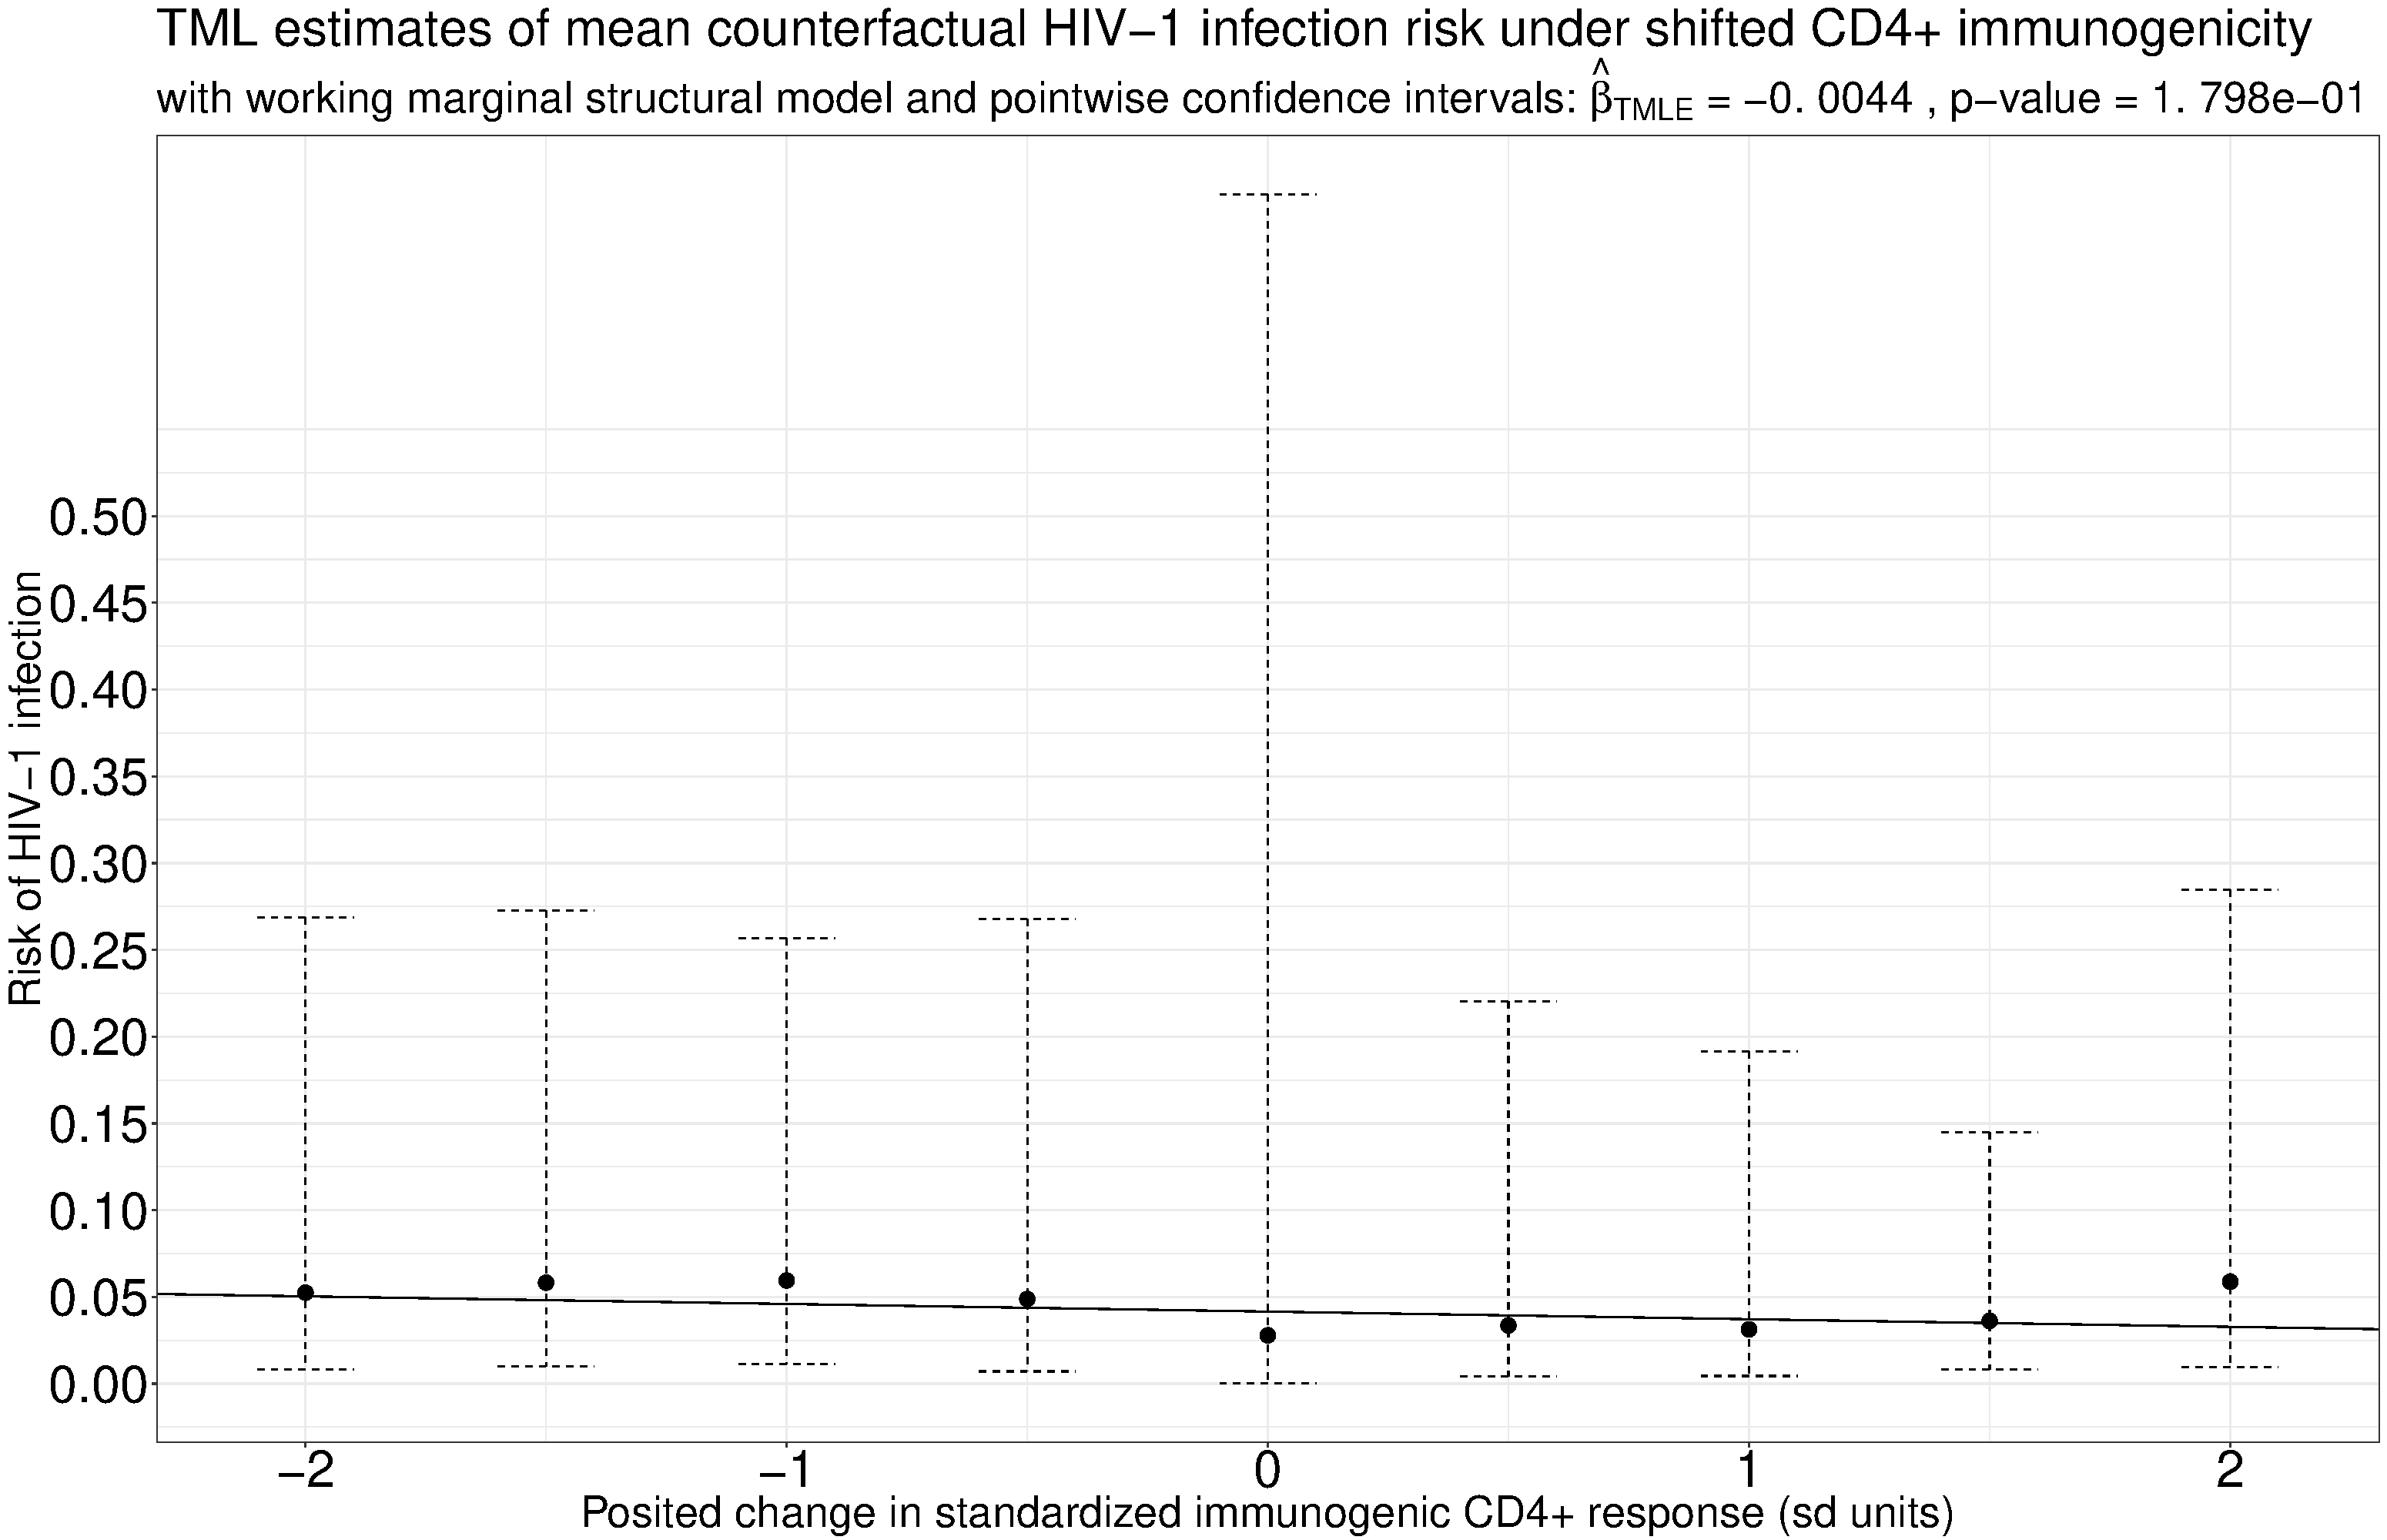
\includegraphics[scale=0.21]{cd4_msm_tmle_summary}
  \caption{
    Analysis of HIV-1 risk as a function of CD4+ immunogenicity, using
    \texttt{R} package \texttt{txshift}
    (\url{https://github.com/nhejazi/txshift}.)
  }
\end{figure}

\note{
}

\end{frame}

%%%%%%%%%%%%%%%%%%%%%%%%%%%%%%%%%%%%%%%%%%%%%%%%%%%%%%%%%%%%%%%%%%%%%%%%%%%%%%%%

\begin{frame}[c]{How does this help in fighting the HIV-1 epidemic? CD8+}

\vspace{-2em}
\begin{figure}[H]
  \centering
  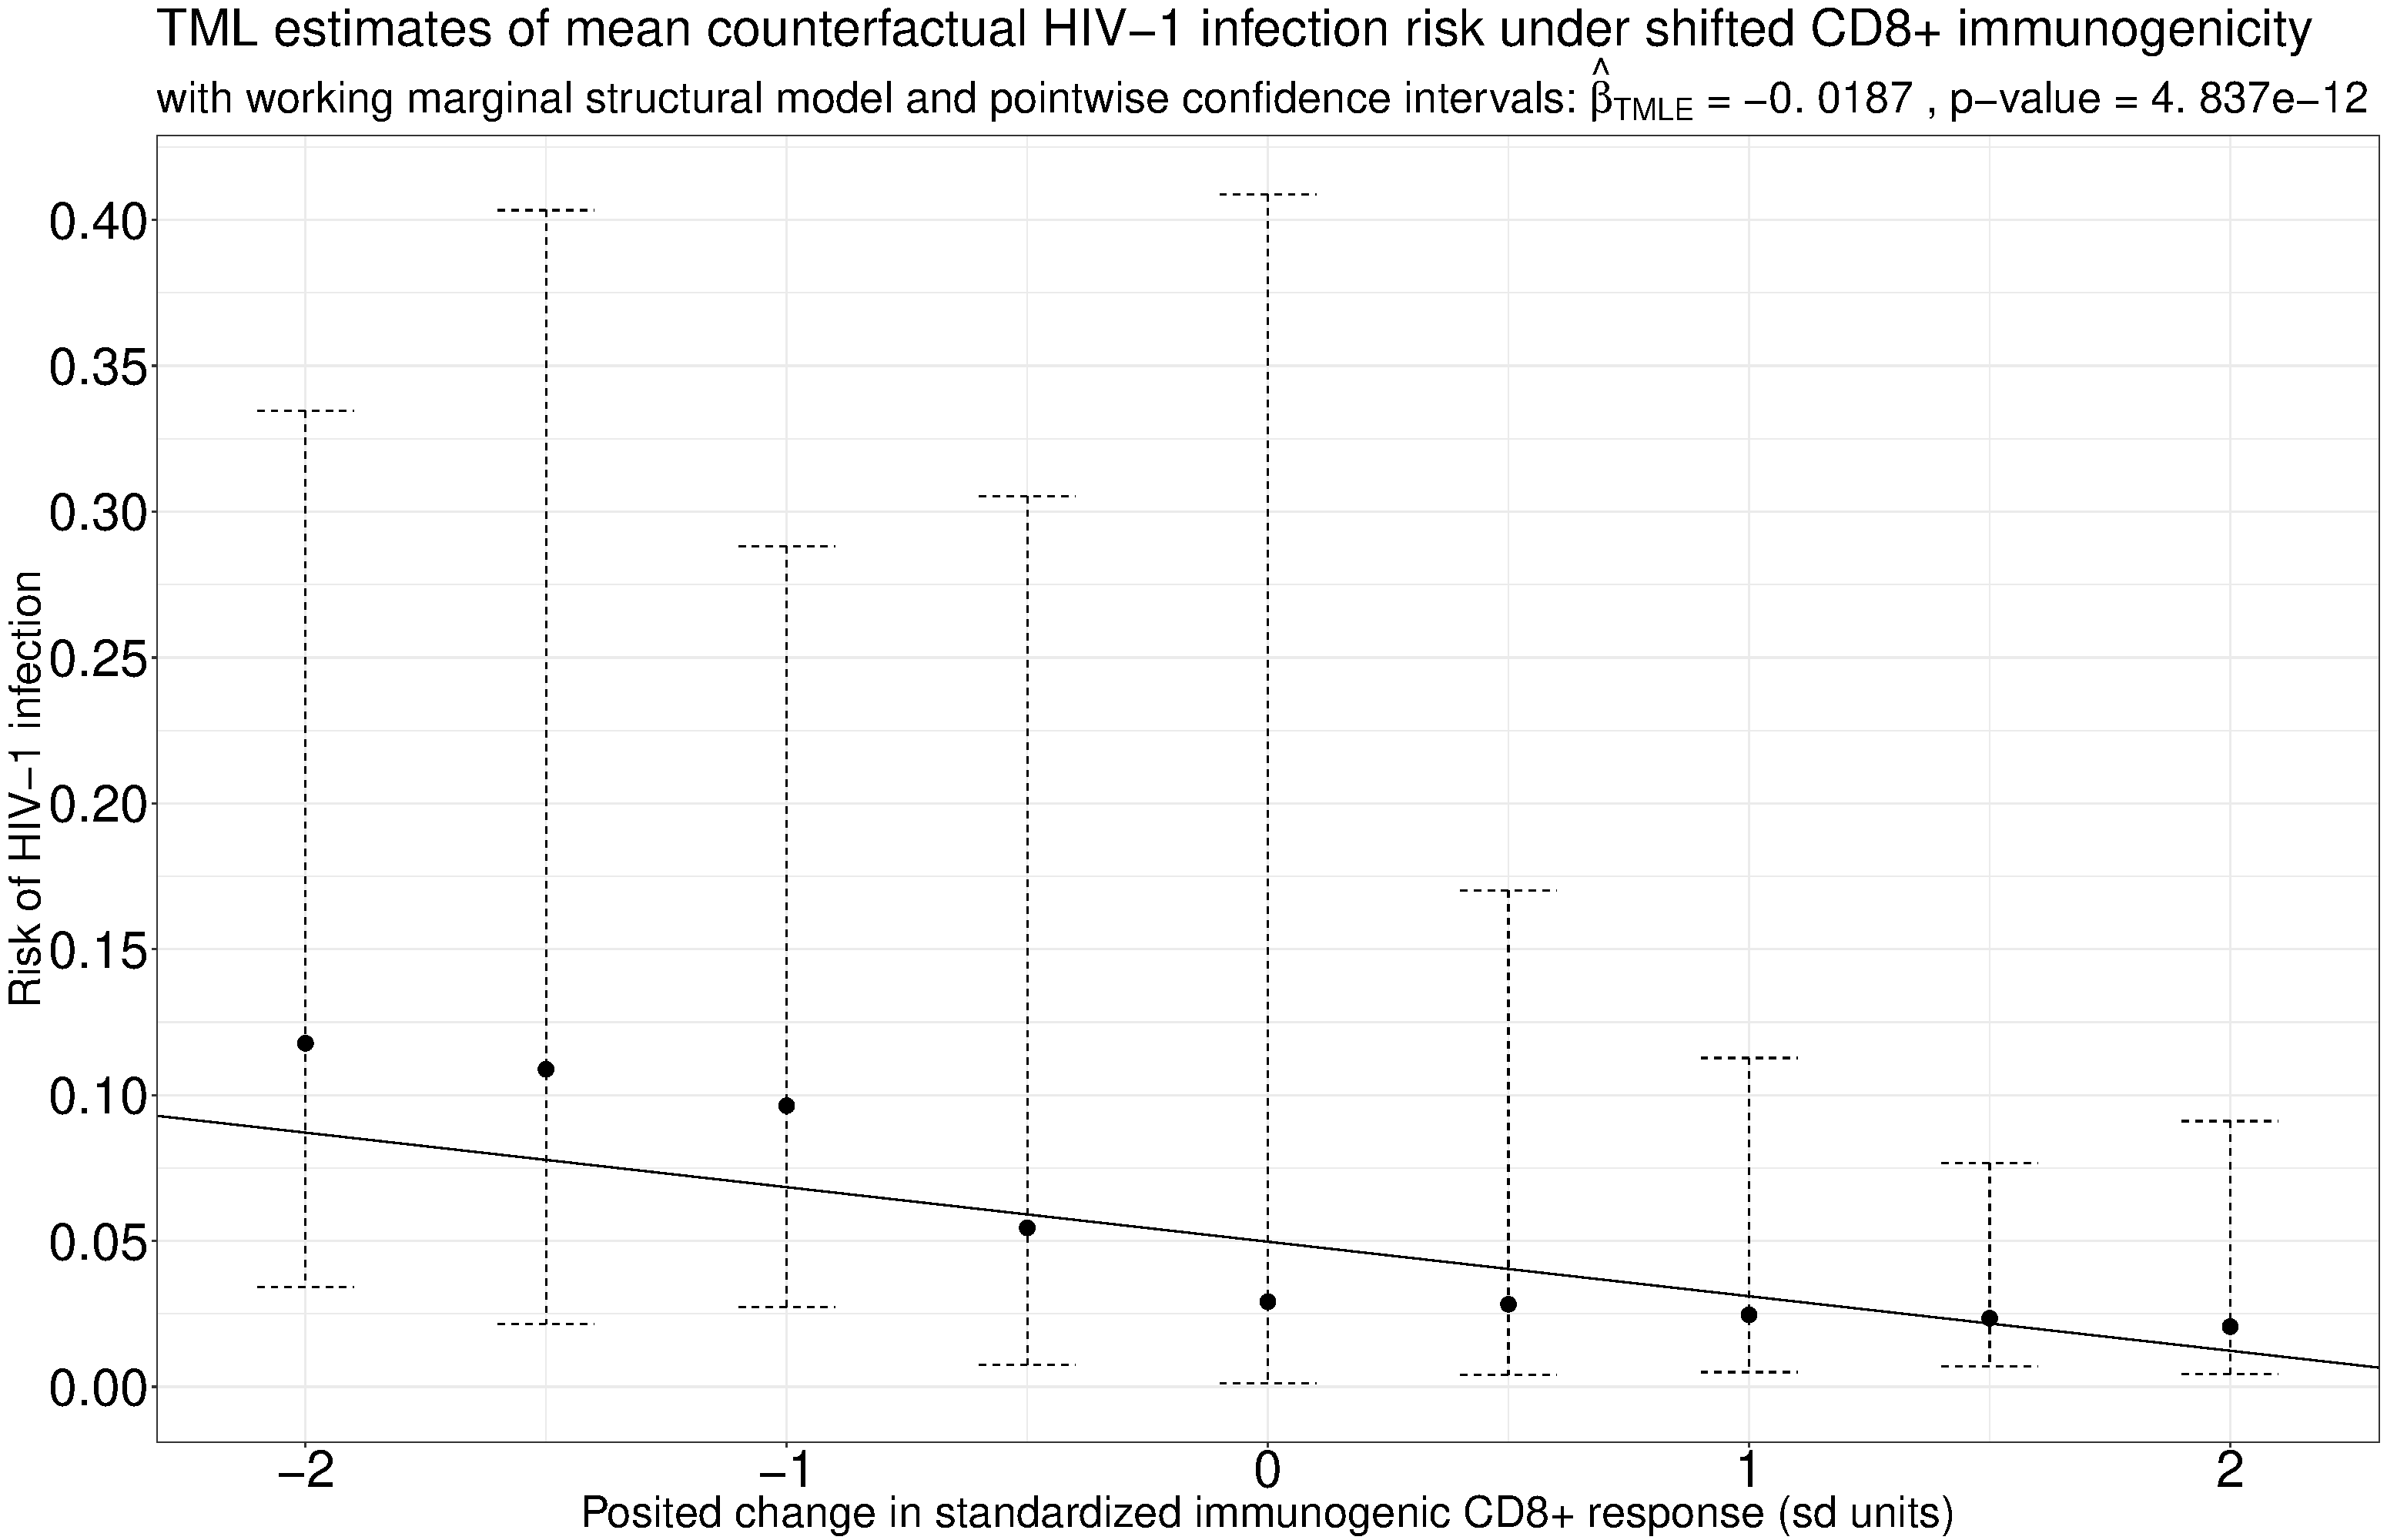
\includegraphics[scale=0.21]{cd8_msm_tmle_summary}
  \caption{
    Analysis of HIV-1 risk as a function of CD8+ immunogenicity, using
    \texttt{R} package \texttt{txshift}
    (\url{https://github.com/nhejazi/txshift}.)
  }
\end{figure}

\note{
}

\end{frame}

%%%%%%%%%%%%%%%%%%%%%%%%%%%%%%%%%%%%%%%%%%%%%%%%%%%%%%%%%%%%%%%%%%%%%%%%%%%%%%%%

\begin{frame}[c]{Efficient and robust estimation under two-phase sampling}

\begin{center}
\begin{itemize}
  \itemsep10pt
  \item We now have a semiparametric-efficient and robust procedure for
    assessing the effect of the intervention $d(a,w) = a + \delta$.
  \item Due to construction based on the IPCW-EIF, any resultant estimators are
    robust and efficient under two-phase sampling.
  \item New \textit{causal} tool for assessing how immunogenic response shifts
    would have affected HIV-1 infection risk.
  \item New open source software for deploying such estimators:
    \begin{itemize}
      \itemsep4pt
      \item \url{https://github.com/nhejazi/haldensify} (densities)
      \item \url{https://github.com/nhejazi/txshift} (AIPW, TMLE)
      \item \url{https://github.com/tlverse/tmle3shift} (TMLE)
    \end {itemize}
\end{itemize}
\end{center}
\note{
}
\end{frame}

%%%%%%%%%%%%%%%%%%%%%%%%%%%%%%%%%%%%%%%%%%%%%%%%%%%%%%%%%%%%%%%%%%%%%%%%%%%%%%%%

% don't want dimming with references
\setbeamercovered{}
\beamerdefaultoverlayspecification{}

\begin{frame}[c,allowframebreaks]{}

\scriptsize
\bibliographystyle{apalike}
\bibliography{references}

\end{frame}

%%%%%%%%%%%%%%%%%%%%%%%%%%%%%%%%%%%%%%%%%%%%%%%%%%%%%%%%%%%%%%%%%%%%%%%%%%%%%%%%

\begin{frame}[c]{Thank you.}

\large
Slides: \href{http://bit.ly/2019\_sfasa\_jsm}{bit.ly/2019\_sfasa\_jsm}
  \quad

\includegraphics[height=4mm]{Figs/cc-zero.png}

\vspace{2mm}
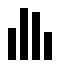
\includegraphics[scale=0.14]{homepage.png} \url{https://nimahejazi.org}

\vspace{2mm}
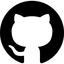
\includegraphics[scale=0.11]{github-icon.png}
  \url{https://github.com/nhejazi}

\vspace{2mm}

\includegraphics[scale=0.14]{twitter-icon.png}
  \url{https://twitter.com/nshejazi}

\end{frame}

%%%%%%%%%%%%%%%%%%%%%%%%%%%%%%%%%%%%%%%%%%%%%%%%%%%%%%%%%%%%%%%%%%%%%%%%%%%%%%%%

\appendix
\begin{frame}[standout]
  Appendix
\end{frame}

%%%%%%%%%%%%%%%%%%%%%%%%%%%%%%%%%%%%%%%%%%%%%%%%%%%%%%%%%%%%%%%%%%%%%%%%%%%%%%%%

\begin{frame}[c]{Nonparametric Conditional Density Estimation}

\begin{center}
\begin{itemize}
  \itemsep8pt
  \item To compute the auxiliary covariate $H(a,w)$, we need to estimate
    conditional densities $g(A \mid W)$ and $g(A - \delta \mid W)$.
  \item There is a rich literature on density estimation, we follow the approach
    proposed in \cite{diaz2011super}.
  \item To build a conditional density estimator, consider
    \begin{equation*}
      g_{n, \alpha}(a \mid W) = \frac{\pr (A \in [\alpha_{t-1}, \alpha_t)
        \mid W)}{\alpha_t - \alpha_{t-1}},
    \end{equation*}
    for $\alpha_{t-1} \leq a < \alpha_t$.
    \vspace{0.5em}
    \begin{itemize}
      \itemsep4pt
      \item This is a classification problem, where we estimate the probability
        that a value of $A$ falls in a bin $[\alpha_{t-1}, \alpha_t)$.
      \item The choice of the tuning parameter $t$ corresponds roughly to the
        choice of bandwidth in classical kernel density estimation.
    \end{itemize}
\end{itemize}
\end{center}

\note{
}

\end{frame}

%%%%%%%%%%%%%%%%%%%%%%%%%%%%%%%%%%%%%%%%%%%%%%%%%%%%%%%%%%%%%%%%%%%%%%%%%%%%%%%%

\begin{frame}[c]{Nonparametric Conditional Density Estimation}

\begin{center}
\begin{itemize}
  \itemsep8pt
  \item \cite{diaz2011super} propose a re-formulation of this classification
    approach as a set of hazard regressions.
  \item To effectively employ this proposed re-formulation, consider
    \begin{align*}
      \pr (A \in [\alpha_{t-1}, \alpha_t) \mid W) =& \pr (A \in [\alpha_{t-1},
      \alpha_t) \mid A \geq \alpha_{t-1}, W) \times  \\ & \Pi_{j = 1}^{t -1}
      \{1 - \pr (A \in [\alpha_{j-1}, \alpha_j) \mid A \geq \alpha_{j-1}, W) \}
    \end{align*}
    \vspace{0.25em}
    \begin{itemize}
      \itemsep4pt
      \item The likelihood of this model may be expressed to correspond to the
        likelihood of a binary variable in a data set expressed via a long-form
        repeated measures structure.
      \item Specifically, the observation of $X_i$ is repeated as many times as
        intervals $[\alpha_{t-1}, \alpha_t)$ are before the interval to which
        $A_i$ belongs, and the binary variables indicating $A_i \in
        [\alpha_{t-1}, \alpha_t)$ are recorded.
    \end{itemize}
\end{itemize}
\end{center}

\note{
}

\end{frame}

%%%%%%%%%%%%%%%%%%%%%%%%%%%%%%%%%%%%%%%%%%%%%%%%%%%%%%%%%%%%%%%%%%%%%%%%%%%%%%%%

\begin{frame}[c]{Density Estimation with the Super Learner Algorithm}

\begin{center}
\begin{itemize}
  \itemsep10pt
  \item To estimate $g(A \mid W$) and $g(A - \delta \mid W)$, use a pooled
    hazard regression, spanning the support of $A$.
  \item We rely on the Super Learner algorithm of \cite{vdl2007super} to build
    an ensemble learner that optimally weights each of the proposed regressions,
    using cross-validation (CV).
  \item The Super Learner algorithm uses $V$-fold CV to train each proposed
    regression model, weighting each by the inverse of its average risk across
    all $V$ holdout sets.
  \item By using a library of regression estimators, we invoke the result of
    \cite{vdl2004asymptotic}, who prove this likelihood-based cross-validated
    estimator to be asymptotically optimal.
\end{itemize}
\end{center}

\note{
\begin{itemize}
  \item The auxiliary covariate simplifies when the treatment is in the limits
    (conditional on $W$) --- i.e., for $A_i \in (u(w) - \delta, u(w))$, then we
    have $H(a,w) = \frac{g_0(a - \delta \mid w)}{g_0(a \mid w)} + 1$.
  \item Asymptotically optimal in the sense that it performs as well as the
    oracle selector as the sample size increases.
\end{itemize}
}

\end{frame}

%%%%%%%%%%%%%%%%%%%%%%%%%%%%%%%%%%%%%%%%%%%%%%%%%%%%%%%%%%%%%%%%%%%%%%%%%%%%%%%%

\begin{frame}[c]{Algorithm for IPCW-TML Estimation}

\begin{center}
\begin{enumerate}\label{ipcwtmle_algo}
  \itemsep8pt
  \item Using all observed units ($X$), estimate sampling mechanism
    $\pi(Y, W)$, perhaps using data-adaptive regression methods.
  \item Using only observed units in the second-stage sample $\Delta = 1$,
    construct initial estimators $g_n(A, W)$ and $\overline{Q}_n(A, W)$,
    weighting by the sampling mechanism estimate $\pi_n(Y, W)$.
  \item With the approach described for the full data case, compute
    $H_n(a_i,w_i)$, and fluctuate submodel via logistic regression.
  \item Compute IPCW-TML estimator $\Psi_n$ of the target parameter, by solving
    the IPCW-augmented EIF estimating equation.
  \item Iteratively update estimated sampling weights $\pi_n(Y,W)$ and
    IPCW-augmented EIF, updating TML estimate in each iteration, until
    $\frac{1}{n}\sum_{i = 1}^n \text{EIF}_i < \frac{1}{n}$.
\end{enumerate}
\end{center}

\note{
  \begin{itemize}
    \item We recommend using nonparametric methods for the initial estimators,
      as consistent estimation is necessary for efficiency of the estimator
      $\Psi_n$.
    \item Intuition for the submodel fluctuation?
    \item This process includes the use of HAL to fit the regression of the EIF
      contributions on the sampling node $\{Y, W\}$.
  \end{itemize}
}

\end{frame}

%%%%%%%%%%%%%%%%%%%%%%%%%%%%%%%%%%%%%%%%%%%%%%%%%%%%%%%%%%%%%%%%%%%%%%%%%%%%%%%%

\end{document}
